%\textsl{}%!TEX TS-options = --shell-escape
%!TEX TS-program = pdflatex
\documentclass[%
   10pt,              % Schriftgroesse
   nenglish,           % wird an andere Pakete weitergereicht
   a4paper,           % Seitengroesse
   DIV11,             % Textbereichsgroesse (siehe Koma Skript Dokumentation !)
]{scrartcl}%     Klassen: scrartcl, scrreprt, scrbook, article
% -------------------------------------------------------------------------

\usepackage[utf8]{inputenc} % Font Encoding, benoetigt fuer Umlaute
\usepackage[english]{babel}   % \textsl{}Spracheinstellung

\usepackage[T1]{fontenc} % T1 Schrift Encoding
\usepackage{textcomp}    % Zusatzliche Symbole (Text Companion font extension)
\usepackage{lmodern,dsfont}     % Latin Modern Schrift
\usepackage{dsfont}
\usepackage{color}
%\usepackage{wasysym}
\usepackage{ulem}
\usepackage{graphicx}
\usepackage{grffile} %allows to use pngs
\usepackage{eurosym}
%\usepackage{txfonts}
\usepackage{stmaryrd}
\usepackage{amsfonts}
\usepackage{amsmath}
\usepackage{hyperref}
\usepackage{tikz}
\usepackage{multirow}
\usepackage{listings}
\usepackage{etextools}
\usepackage{ifthen}
\usepackage{cite}
%\usepackage{TikZ} %phylogenetischer Baum
%\usetikzlibrary{calc, shapes, backgrounds} %für die Phylogenetische bäume
%\usetikzlibrary{automata,arrows}
\usepackage{subfigure} 


% Definition des Headers
\usepackage{geometry}
\geometry{a4paper, top=3cm, left=3cm, right=3cm, bottom=3cm, headsep=0mm, footskip=0mm}
\renewcommand{\baselinestretch}{1.3}\normalsize

\def\header#1#2#3#4#5#6#7{\pagestyle{empty}
\noindent
\begin{minipage}[t]{0.6\textwidth}
\begin{flushleft}
\textbf{#4}\\% Fach
#6\\% Semester
Tutor: #2  % Tutor 
\end{flushleft}
\end{minipage}
\begin{minipage}[t]{0.4\textwidth}
\begin{flushright}
\points{#7}% Punktetabelle
\vspace*{0.2cm}
#5%  Names
\end{flushright}
\end{minipage}

\begin{center}
{\Large\textbf{ Assignment #1}} % Blatt

{(Abgabe am #3)} % Abgabedatum
\end{center}
}

\newenvironment{vartab}[1]
{
    \begin{tabular}{ |c@{} *{#1}{c|} } %\hline
}{
    \end{tabular}
}

\newcommand{\myformat}[1]{& #1}

\newcommand{\entry}[1]{
  \edef\result{\csvloop[\myformat]{#1}}
  \result \\ \hline
}

\newcommand{\numbers}[1]{
  \newcounter{ctra}
\setcounter{ctra}{1}
\whiledo {\value{ctra} < #1}%
{%
  \myformat{\thectra}
  \stepcounter{ctra}%
}
\myformat{\thectra}
}
\newcommand{\emptyLine}[1]{
  \newcounter{ctra1}
\setcounter{ctra}{1}
\whiledo {\value{ctra1} < #1}%
{%
  \myformat{\hspace*{0.5cm}}
  \stepcounter{ctra1}%
}
}

\newcommand{\points}[1]{
\newcounter{colmns}
\setcounter{colmns}{#1}
\stepcounter{colmns}
  \begin{vartab}{\thecolmns}
    \numbers{#1} & $\sum$\\\hline
    \emptyLine{\thecolmns}\\
  \end{vartab}
}


\begin{document}
%\header{Blatt}{Tutor}{Abgabedatum}{Vorlesung}{Bearbeiter}{Semester}{Anzahl Aufgaben}
\header{4}{Alexander Seitz}{9. November 2015}{Bioinformatics I}{\\Jonas Ditz \\\& Benjamin Schroeder}{WS 15/16}{3}

\section*{Theoretical Assignment - \textsl{Optimal multiple alignment}}

To calculate our MSA we use the recursion written down on page 50 in the script. 

\begin{equation}
 F(i_1, i_2, i_3) = max \begin{cases}
                         F(i_1 -1, i_2 -1, i_3 -1) + s_{SP}(a_{1i_1},a_{2i_2},a_{3i_3}) \\
                         \\
                         F(i_1 -1, i_2 -1, i_3) + s_{SP}(a_{1i_1},a_{2i_2},-) \\
                         F(i_1 -1, i_2, i_3 -1) + s_{SP}(a_{1i_1},-,a_{3i_3}) \\
                         F(i_1, i_2 -1, i_3 -1) + s_{SP}(-,a_{2i_2},a_{3i_3}) \\
                         \\
                         F(i_1 -1, i_2, i_3) + s_{SP}(a_{1i_1},-,-) \\
                         F(i_1, i_2 -1, i_3) + s_{SP}(-,a_{2i_2},-) \\
                         F(i_1, i_2, i_3 -1) + s_{SP}(-,-,a_{3i_3}) \\
                        \end{cases} \nonumber
\end{equation}

\noindent Such a recursion results in a three-dimensional matrix. Since such a matrix is really difficult to 
sketch, we split it into three two-dimensional matrices.  

\begin{figure}[ht]
\centering
\subfigure{
\begin{tabular}{c|cccc}
 0 & 0 & C & C & T \\
 \hline
 0 & \textcolor{red}{\textbf{0}} & -2 & -4 & -6 \\
 C & -2 & \textcolor{red}{\textbf{-2}} & -4 & -10 \\
 T & -4 & -8 & -8 & -6 \\
 T & -6 & -10 & -12 & -10 \\
\end{tabular}}
\subfigure{
\begin{tabular}{c|cccc}
 T & 0 & C & C & T \\
 \hline
 0 & -2 & -4 & -6 & -8 \\
 C & -4 & -4 & -6 & -10 \\
 T & -6 & -8 & \textcolor{red}{\textbf{-4}} & 2 \\
 T & -8 & -10 & -8 & 2 \\
\end{tabular}}
\subfigure{
\begin{tabular}{c|cccc}
 C & 0 & C & C & T \\
 \hline
 0 & -4 & -6 & -8 & -10 \\
 C & -6 & 2 & 2 & -8 \\
 T & -8 & -6 & -2 & 0 \\
 T & -10 & -8 & -6 & \textcolor{red}{\textbf{-6}} \\
\end{tabular}}
\caption[DP matrix of MSA]{DP matrix of MSA, traceback is shown in red}
\end{figure}

\noindent If we fill the DP matrix using this recursion, we get several optimal alignments. One of 
them is the following:

\begin{equation}
 \begin{pmatrix}
  C & T & T \\
  - & T & C \\
  C & C & T
 \end{pmatrix}
\end{equation}

\noindent with score $\alpha_{SP}(A^*) = S(A,B) + S(A,C) + S(B,C) = -2 + 2 + (-6) = -6$.


\section*{Theoretical Assignment - \textsl{Progressive alignment}}
Progressive alignment methodes are one way to create multiple sequence alignments (MSA), in this task we had to accomplish manualy a progressive alignment. The first step for the progressive alignment was to generate the pairwise global distance matrices. Afterwards the global optima were entered into a new table, which was used to generate the guide tree in the second step.(figure \ref{DP2}).
\begin{figure}[ht]
        \centering
	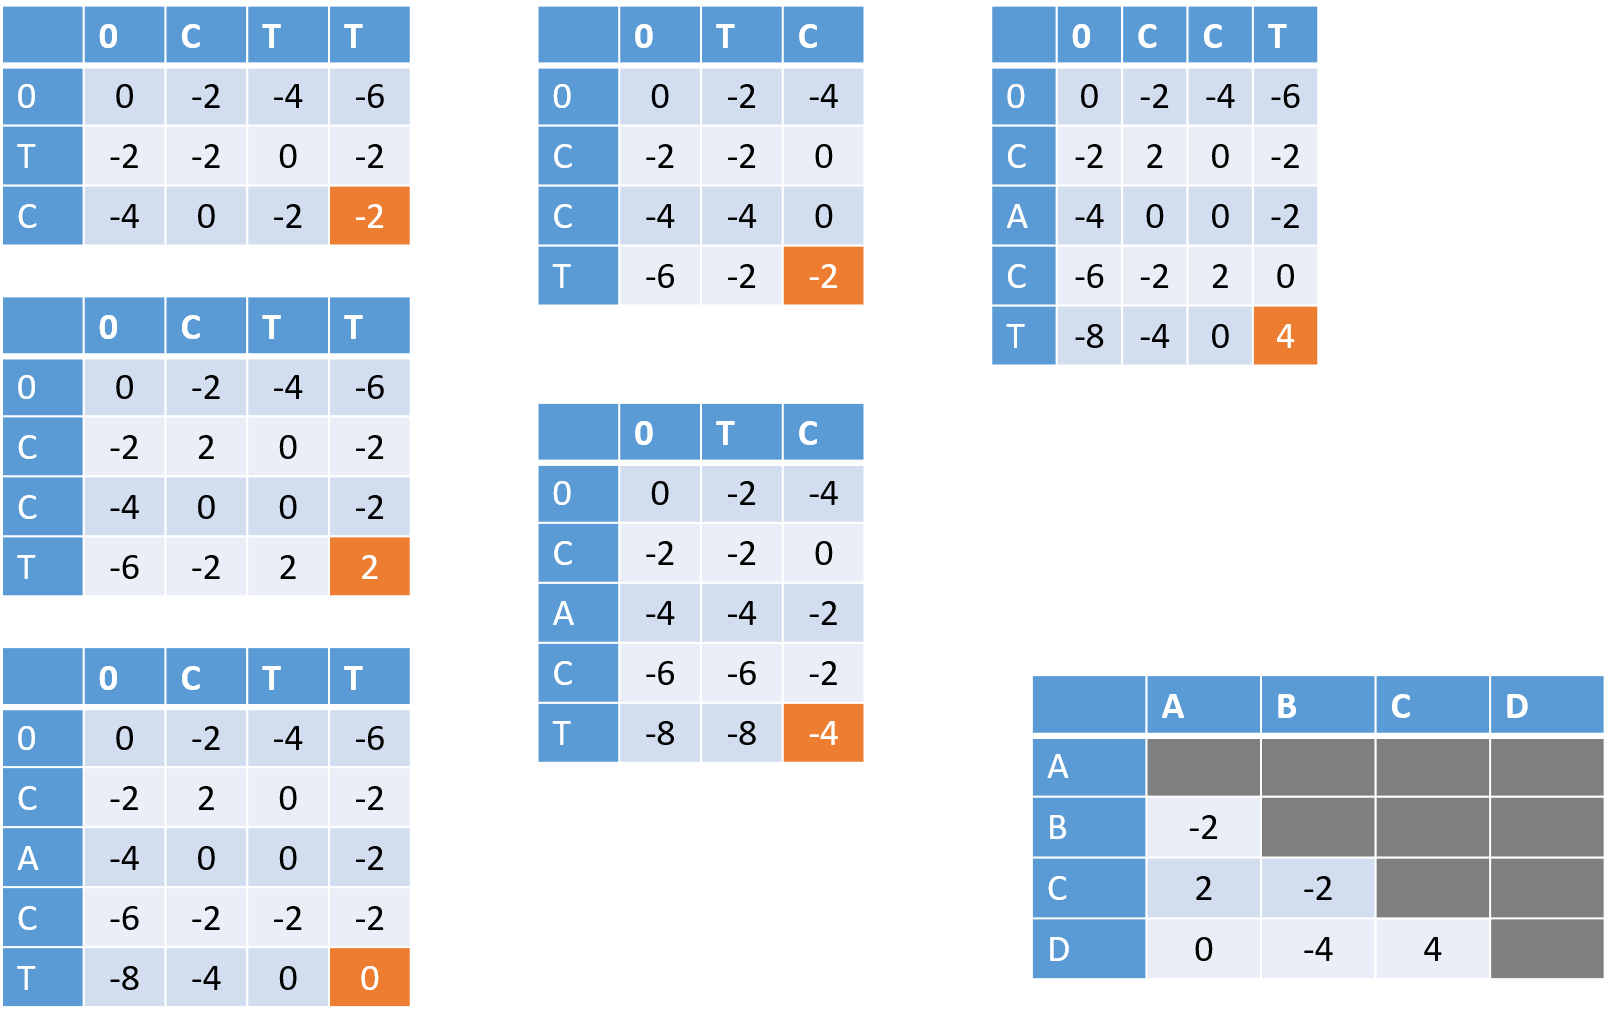
\includegraphics[width=0.7\textwidth]{Img/Exercise2-DP-Matrix.png}
	\caption{ Global alignments lead to the basis table used to generate the guide tree}
	\label{DP2}
\end{figure}

In step 2 the guide tree was created by the UPGMA methode in 3 substeps. After every step, which added a new cluster, the distance table was updated. The result from this step was the guide tree, which was used to apply the 'complete alignment' methode in the last step, the progressive alignment step.(figure \ref{guidetree2})


\begin{figure}[ht]
        \centering
	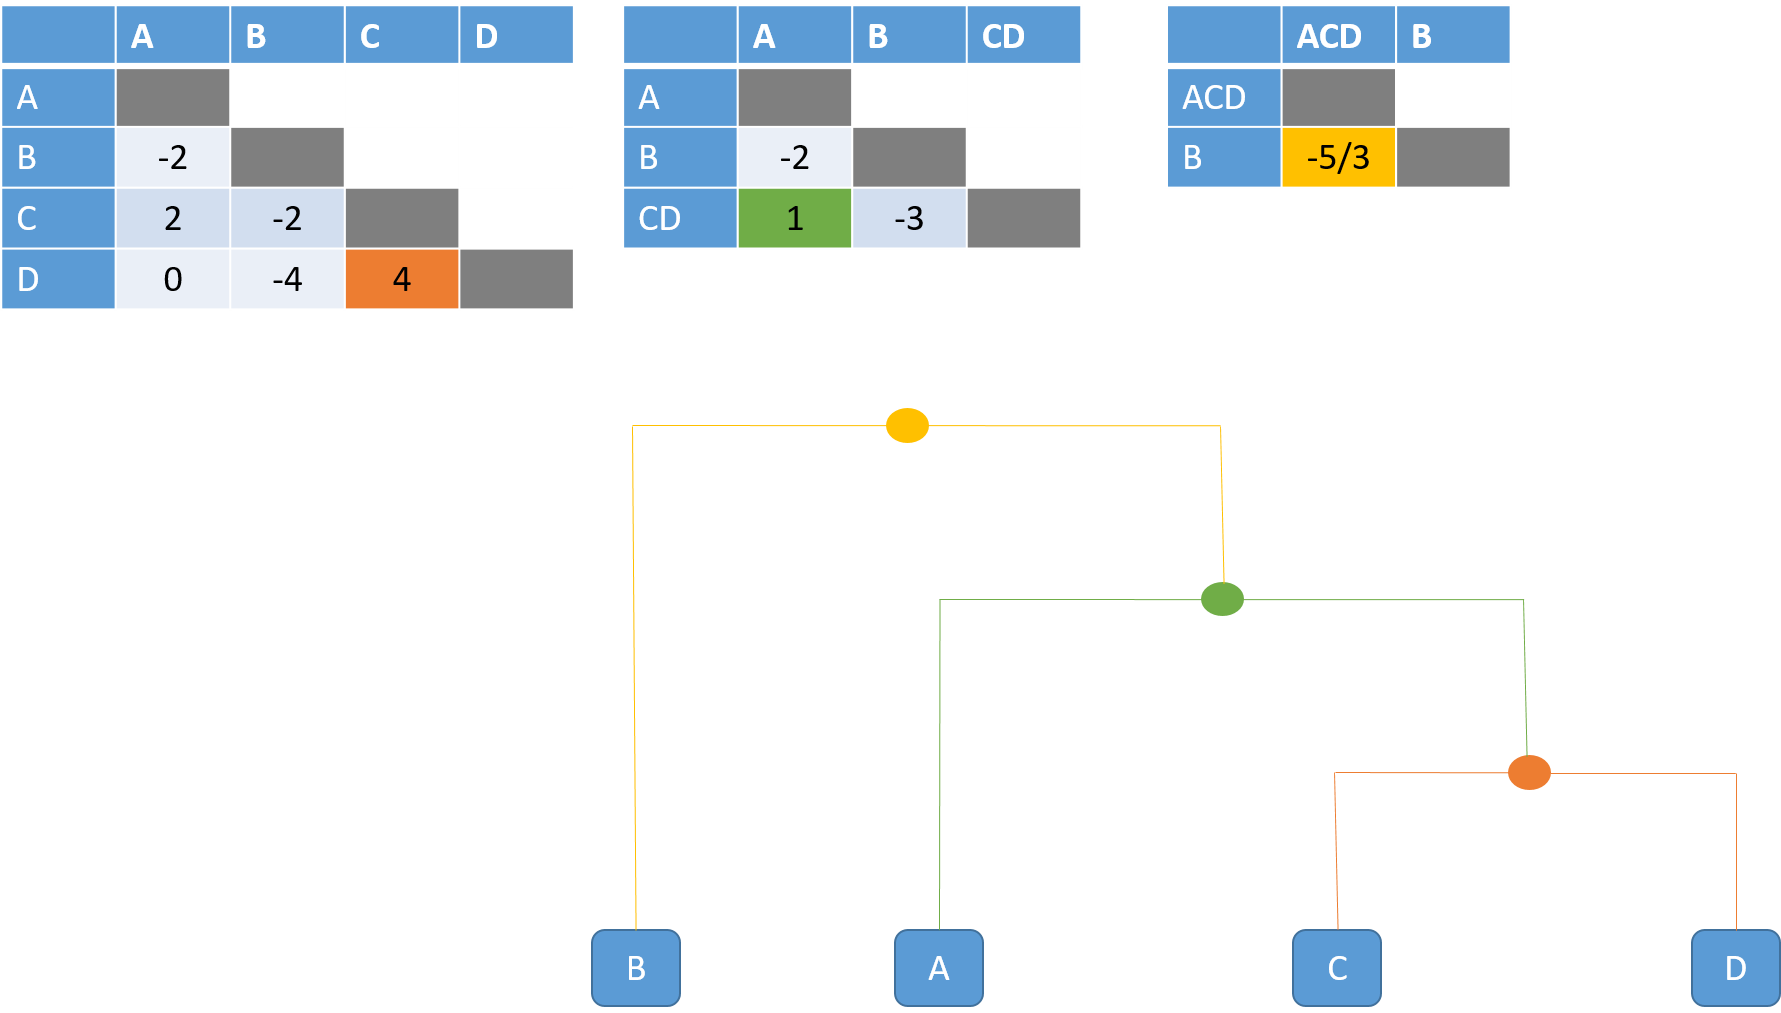
\includegraphics[width=0.7\textwidth]{Img/Exercise2-Guidetree.png}
	\caption{ The guide tree is made from the final table from step 1}
	\label{guidetree2}
\end{figure}

The last step was creating the actual MSA. The 'complete alignment' methode was used. This means after every step, the distance of the new sequences was determined to each other sequence in the cluster. The optimal resulting score was used to get the best alignment for the new Sequence. after 3 steps the MSA was completed. (figure \ref{completealign})
\begin{figure}[ht]
        \centering
	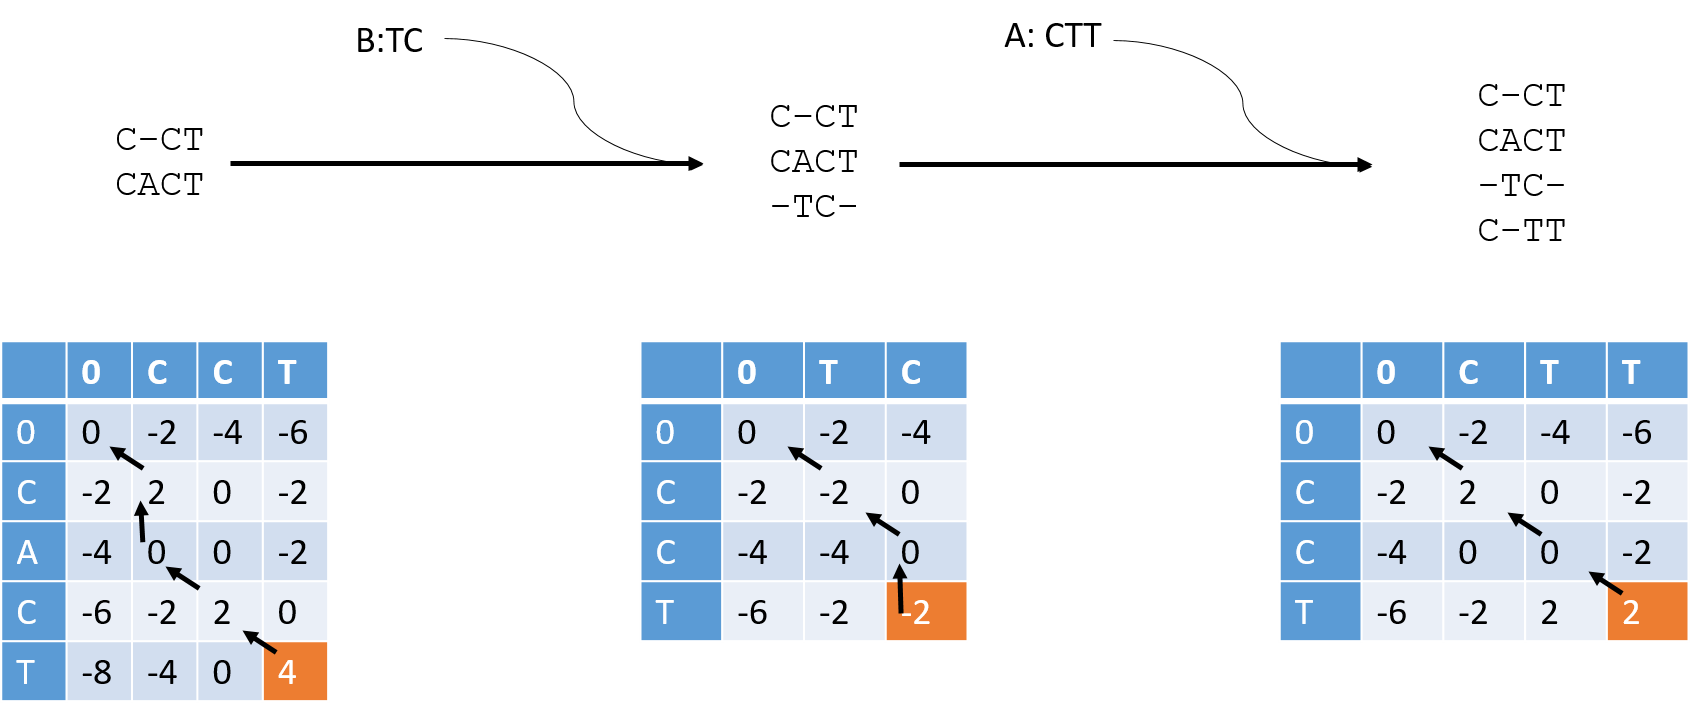
\includegraphics[width=0.7\textwidth]{Img/Exercise2-CompleteAlignment.png}
	\caption{ Complete alignment methode is used to get an MSA from the guidetree from step 2	}
	\label{completealign}
\end{figure}


\section*{Practical Assignment - \textsl{Comparing multiple alignment}}
Multiple sequence alignments (MSA) are very important to detect similarities between several 
sequences and e.g. determine whether a sequence belongs to a certain family or not. Hence, many 
different programs, such as ClustalW, were developed to calculate a MSA. We calculated a multiple 
sequence alignment for three files (BB11007, BB20002 and Prolyl-tRNA), each file contained several 
sequences, with different programs 
to compare the results. The used programs are Clustal$\Omega$\cite{Sievers539}, MAFFT\cite{Katoh1} 
and MUSCLE\cite{Edgar1, Edgar2}. The resulting MSAs were compared with a gold standard provided by 
BaliBase\cite{Bahr1}. This database provide a large number of reference MSAs as well as a program 
\grqq BaliScore\grqq , which can be used to calculate different scores to evaluate your MSA. For 
this assignment we are interested in the total column score, which is the percentage of accurately 
reconstructed columns of the reference MSA, and the sum-of-pair score, which is for BaliScore the 
percentage of pairs of aligned residues that are similar in the reference and the reconstructed 
MSA. Furthermore, a important information is the runtime of different programs. We used the bash 
command \textit{time} to collect this information.\\
\\
\noindent Clustal$\Omega$ is the newest extension for the Clustal family. One problem of ClustalW 
was the scalability. With Clustal$\Omega$ a MSA can now calculated for hundreds of thousands of 
sequences within a few hours. On the technical side the algorithm can use multiple processors. 
According to the official site\footnote{http://www.clustal.org/omega/}, Clustal$\Omega$ produces 
better alignments than previous versions. MAFFT offers several modes. The L-INS-i mode is 
slower and only suitable for alignments with less than 200 sequences but results in a more accurate 
alignment. Contrary to that mode the FFT-NS-2 mode can be used to align up to 300.000 sequences. It 
is a lot faster by using the Fast Fourier Transformation but also less accurate. We used the 
FFT-NS-2 mode for this assignment. The third program MUSCLE is a iterative approach to multiple 
sequence alignments. It uses a very accurate distance measure two calculate relatedness of two 
sequences and updates this distance measure for every iteration step.\\
\\
\noindent The resulting total column scores can be found in figure \ref{totCol}. All calculated sum-
of-pairs scores are written down in figure \ref{SPscore} and the runtime of all programs can be found 
in figure \ref{runtime}. 


\begin{figure}[ht]
 \centering
 \subfigure{
 \begin{tabular}{c|ccc}
  \textit{total column score} & \textbf{Clustal$\Omega$} & \textbf{MUSCLE} & \textbf{MAFFT} \\
  \hline
  \textbf{BB11007} & 0.33 & 0.39 & 0.24 \\
  \textbf{BB20002} & 0.00 & 0.00 & 0.00 \\
  \textbf{Prolyl-tRNA} & $c_{1,3}$ & $c_{2,3}$ & $c_{3,3}$ \\
 \end{tabular}}
 \caption{total column score of all alignments}
 \label{totCol}
\end{figure}

\begin{figure}[ht]
 \centering
 \subfigure{
 \begin{tabular}{c|ccc}
   \textit{SP-score}& \textbf{Clustal$\Omega$} & \textbf{MUSCLE} & \textbf{MAFFT} \\
  \hline
  \textbf{BB11007} & 0.597 & 0.582 & 0.524 \\
  \textbf{BB20002} & 0.314 & 0.197 & 0.246 \\
  \textbf{Prolyl-tRNA} & $s_{1,3}$ & $s_{2,3}$ & $s_{3,3}$ \\
 \end{tabular}}
 \caption{sum-of-pairs score of all alignments}
 \label{SPscore}
\end{figure}

\begin{figure}[ht]
 \centering
 \subfigure{
 \begin{tabular}{c|ccc}
  \textit{runtime} & \textbf{Clustal$\Omega$} & \textbf{MUSCLE} & \textbf{MAFFT} \\
  \hline
  \textbf{BB11007} & 0.389 & 0.488 & 0.13 \\
  \textbf{BB20002} & 6.62 & 19.928 & 0.38 \\
  \textbf{Prolyl-tRNA} & $t_{1,3}$ & $t_{2,3}$ & $t_{3,3}$ \\
 \end{tabular}}
 \caption{runtime of all used programs for example files (in sec)}
 \label{runtime}
\end{figure}

\newpage
\bibliography{Assignment4-Ditz_Schroeder-WS15-16.bib}
\bibliographystyle{ieeetr}
 
\end{document}